\section{Төлөөллийн загварыг үүсгэх}
\begin{figure}[ht]
	\centering
	\begin{subfigure}{\textwidth/2}
		\centering
		
\includegraphics[width=\textwidth-1cm]{./images/DrawTree.png}
		\caption{BSP}
		\label{fig:DrawTree}
	\end{subfigure}%
	\begin{subfigure}{\textwidth/2}
		\centering
		
\includegraphics[width=\textwidth-1cm]{./images/ProceduralDungeonTestWall.png}
		\caption{Хануудыг тодорхойлсон GridXZ}
		\label{fig:ProceduralDungeonTestWall}
	\end{subfigure}
	\caption{Үр дүнгийн загвар}
	\label{fig:Results1}
\end{figure}
\subsection{BSP}
BSP-г тодорхойлноор төлөөллийн загварын буюу орчны өрөөнүүдийн ерөнхий бүтцийг гаргана. Өөр өнгийн тэгш өнцөгтүүд нь өөр өөр өрөөнүүдийг илтгэнэ \ref{fig:DrawTree}.

\subsection{GridXZ-н GridCell-үүдэд Wall төрлийг оноох}
Өрөө болгоны ханыг тодорхойлно. Цэнхэр хэсэг нь Wall төрөлтэй GridCell-г загварчилж байна \ref{fig:ProceduralDungeonTestWall}.

\begin{figure}[ht]
	\centering
	\begin{subfigure}{\textwidth/2}
		\centering
		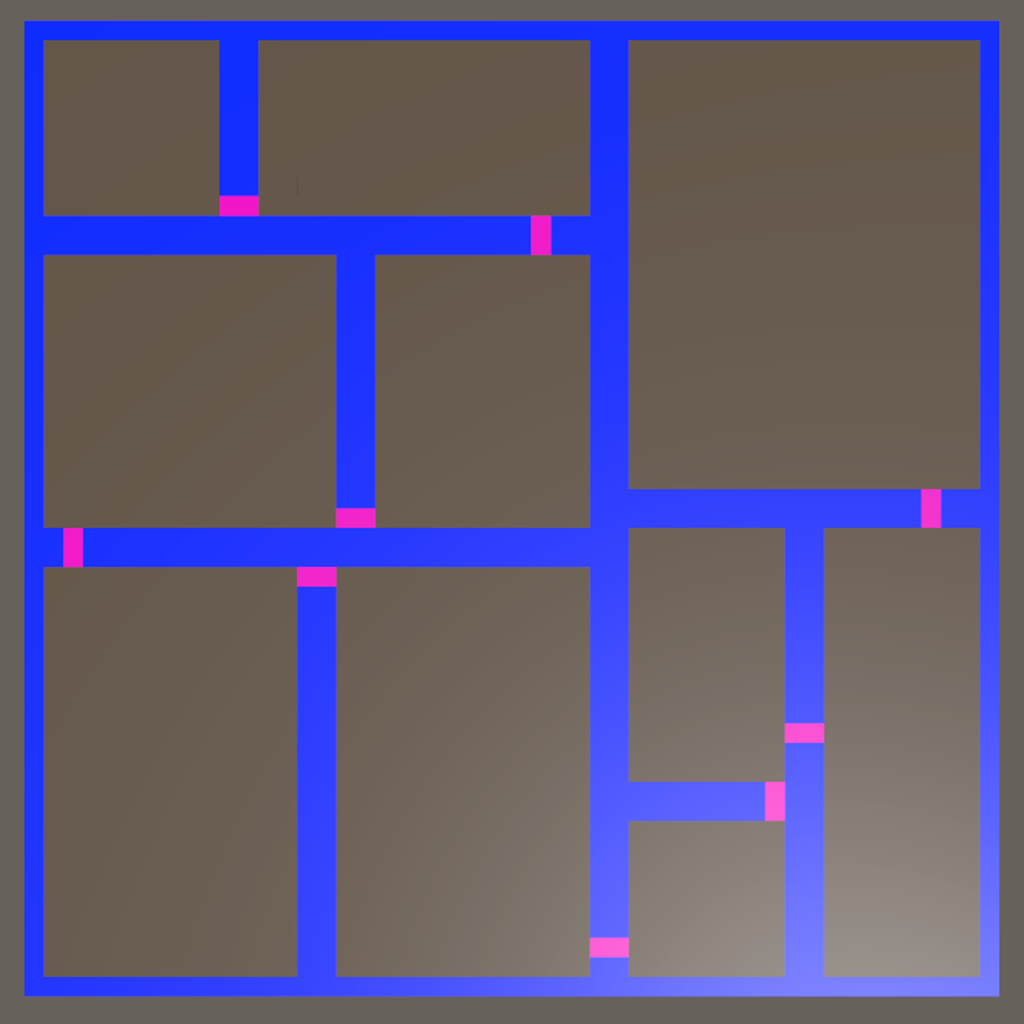
\includegraphics[width=\textwidth-1cm]{./images/ProceduralDungeonTestWallDoor.png}
		\caption{Хана, хаалгуудыг тодорхойлсон GridXZ}
		\label{fig:ProceduralDungeonTestWallDoor}
	\end{subfigure}%
	\begin{subfigure}{\textwidth/2}
		\centering
		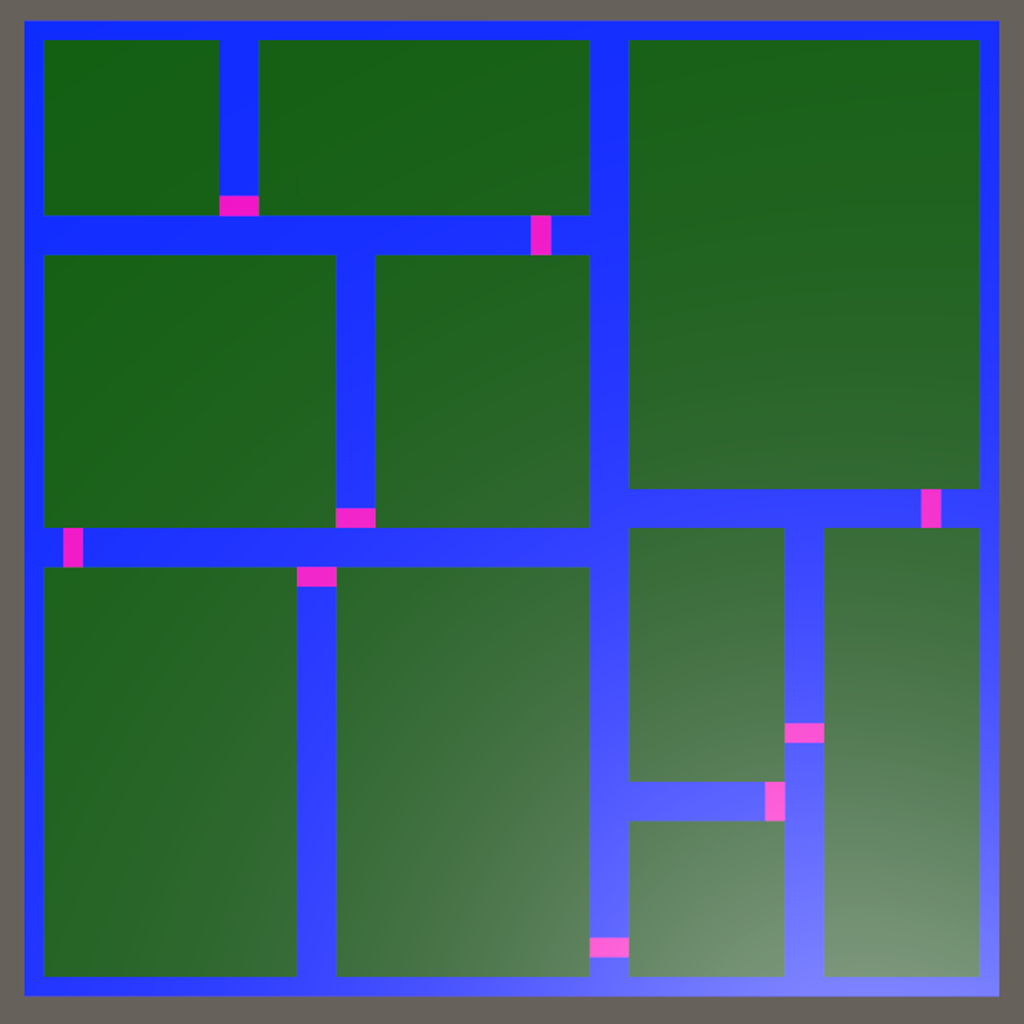
\includegraphics[width=\textwidth-1cm]{./images/ProceduralDungeonTestWallDoorFloor.png}
		\caption{Хана, хаалга, шалыг тодорхойлсон GridXZ}
		\label{fig:ProceduralDungeonTestWallDoorFloor}
	\end{subfigure}
	\caption{Үр дүнгийн загвар}
	\label{fig:Results2}
\end{figure}

\subsection{GridXZ-н GridCell-үүдэд Door төрлийг оноох}
Өрөө болгоны хаалгыг тодорхойлно. BSP-г ашиглаж хаалганы оноолтыг хийх ба аль ч өрөөнөөс аль ч өрөө рүү шилжих боломжтой, өрөө болгох нь хоёр хаалгатай. Хаалганы нэгжийг ягаан өнгөөр дүрлэв \ref{fig:ProceduralDungeonTestWallDoor}
\subsection{GridXZ-н GridCell-үүдэд Floor төрлийг оноох}
Орчны төлөөллийн загварын шалыг тодорхойлж байна. Ногоон өнгөөр дүрслэв \ref{fig:ProceduralDungeonTestWallDoorFloor}.

\section{Тоглоомын моделийг үүсгэх}
\begin{figure}[ht]
	\centering
	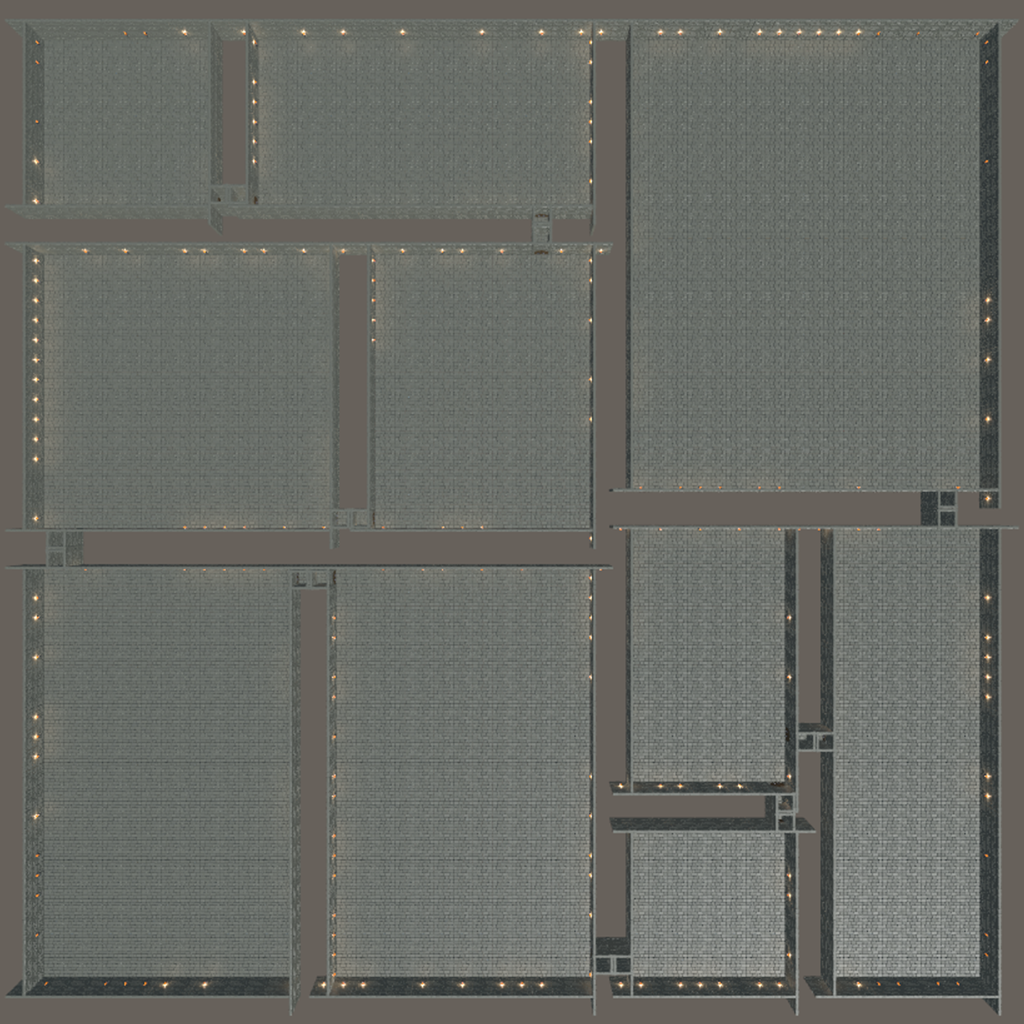
\includegraphics[width=\textwidth-2cm]{./images/Procedural Dungeon.png}
	\caption{Тоглоомын орчин}
	\label{fig:ProceduralDungeon}
\end{figure}
Төлөөллийн загварт суурилж тоглоомын орчинг үүсгэв \ref{fig:ProceduralDungeon}.

\section{CellUnit, CellBundle үүсгэх.}
Хэрэглэгч эсвэл хөгжүүлэгч нь системийг ашиглахдаа шинээр CellBundle болон үүнд хамаарах CellUnit-уудыг үүсгэх боломжтой ба дараах байдлаар үүсгэнэ.

\subsection{CellBundle үүсгэх}
\begin{enumerate}
	\item Шинээр \textit{CellBundle} үүсгэнэ.
	\item Өрөөний хамгийн жижиг байх хэмжээг \textit{MIN\_ROOM\_SIZE}-д оноож өгнө.
	\item Өрөөний хамгийн том байх хэмжээг \textit{MAX\_ROOM\_SIZE}-д оноож өгнө.
	\item BSP-н нүд мутацлах боломжийг \textit{LEAF\_NODE\_CHANCE}-д оноож өгнө.
	\item Тухайн \textit{CellBundle}-н нэрийг Bundle Name-д оноож өнгө.
	\item \textit{Floor, Wall, Pillar, Abyss, Stair Down, Stair Up, Door} гэсэн жагсаалтын оролтын хэсэгт хэрэглэгч хамаарах \textit{CellUnit}-уудыг оноож өгнө.
\end{enumerate}

\begin{figure}[b]
	\centering
	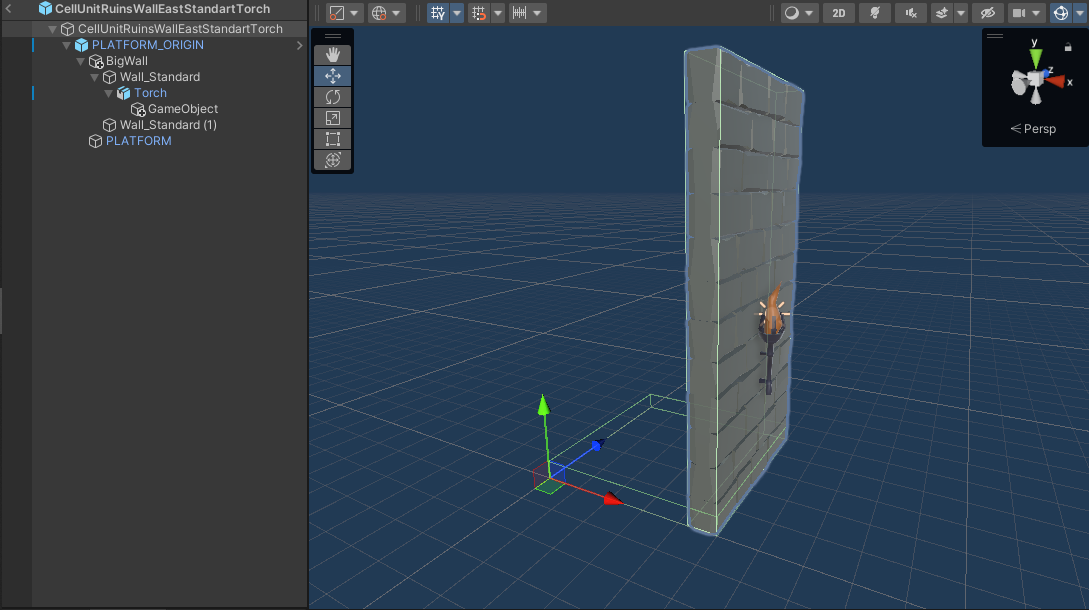
\includegraphics[width=\textwidth-2cm]{./images/CellUnit.png}
	\caption{CellUnit-г тодорхойлж буй жишээ}
	\label{fig:CellUnit}
\end{figure}
\subsection{CellUnit үүсгэх}
\begin{enumerate}
	\item \textit{PLATFORM\_ORIGIN} prefab-г ашиглан \textit{PLATFORM}-д харьяалагдах хэсгийг Зураг \ref{fig:CellUnit}-н дагуу тодорхойлж өгнө.
	\item \textit{PLATFORM\_ORIGIN} нь \textit{PLATFORM} GameObject-г агуулсан prefab.
	\item \textit{PLATFORM} нь тухайн нэгжийн хязраарыг тодорхойлох collider component-тэй GameObject.
\end{enumerate}

\section{Хэрэглэгчийн тест, сайжруулалт.}
Хэрэглэгчийн тест хийх явцад BSP-н навч биш нүд хоорондын коридорыг тодорхойлоход корридор нь өөр өрөөрүү биш хаалганы CellUnit гарах үр дүнг үүсгэх тохиолдол байсан. Энэ нь хүсэмжгүй үр дүн ба хаалга нь өөр өрөөрүү заавал харсан байх хэрэгтэй. Систем нь процедурт программчлалаар зохиогдсон учир орчны төлөөллийн загварын хаалгыг үүсгэх хэсэгт алдаа байгааг амархнаар илрүүлж чадсан.
\subsection{Алдаа}
Хаалганы байршил өрөөрүү бус корридорруу харах хэлбэрээр үүсэх шалтгаан нь навч өрөөнүүдийн хооронд хаалганы CellUnit-г үүсгэхдээ өөр корридорруу харахгүй байршилд үүсгэх дүрмийг тодорхойлж өгсөн ч эцэг нүд хоорондын хаалганы CellUnit-г тодорхойлохдоо үүнийг тодорхойлоогүй орхисон байв.
\subsection{Засвар}
Засварыг хийхдээ кодод Зураг \ref{fig:fix}-н дагуу өөрчлөлт оруулав. Дахин хэрэглэгчийн тестийг олон удаа хийхэд энэ алдаа гараагүй.
\begin{figure}[t]
	\centering
	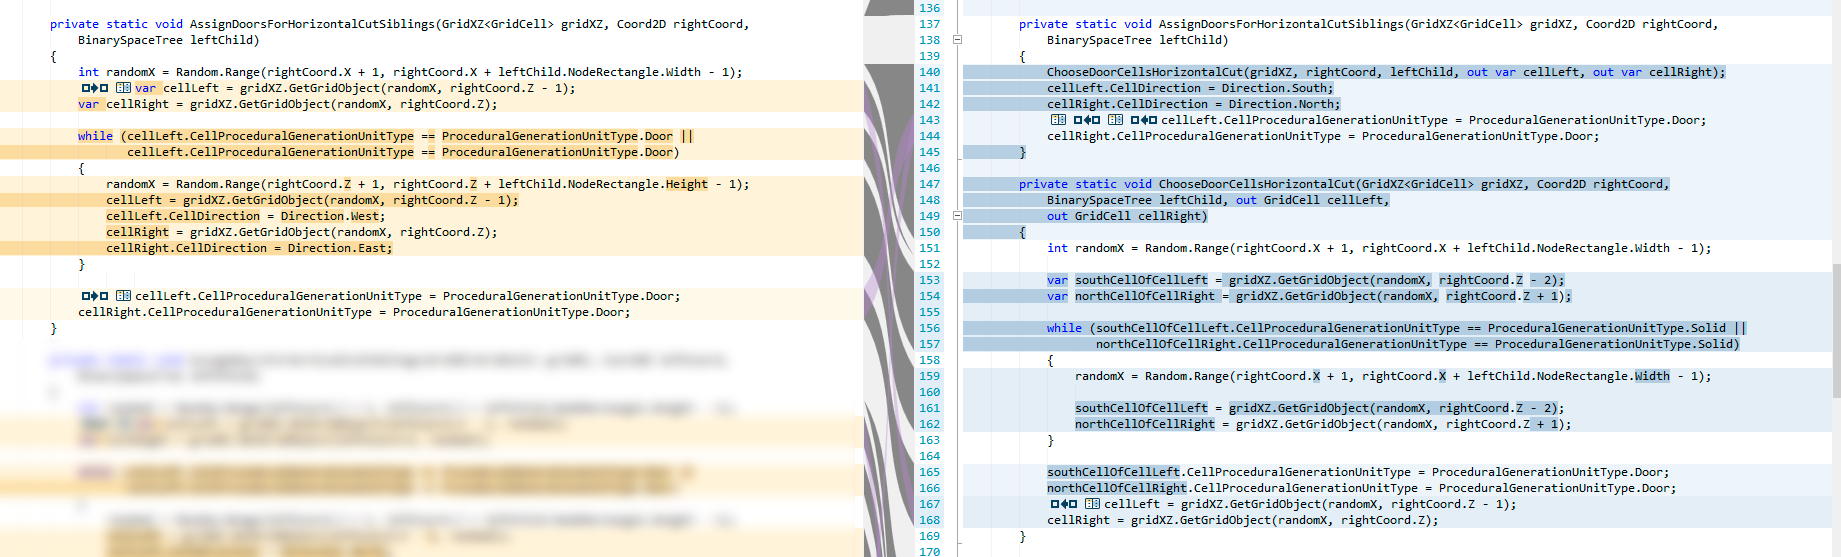
\includegraphics[width=\textwidth]{./images/fix.png}
	\caption{Хаалга CellUnit-н алдааны засвар}
	\label{fig:fix}
\end{figure}

\section{Хэлэлцүүлэг}
Аливаа төвөгтэй процедурт үүсгэлтийг хэрэгжүүлэхдээ боловсруулалтыг үе шаттай хийвэл системийг өргөжүүлэх, өөрчлөлт оруулахад тустай байв. Өөрөөр хэлбэл функциональ хандлагаар олон модулиуд боловсруулалт дараалан хийнэ. Ингэхийн тулд хөгжүүлэгч модулиудын хоорондын харилцаа, оролт гаралтыг тодорхойлсон байх шаардлагатай ба хамгийн түрүүнд хөгжүүлэгч хүссэн үр дүнгээ тодорхойлсон байх ёстой. Аливаа процедурт үүсгэлтийн системийн доторх модулиудын өөр олон төрлийг харин объект хандлагаар хэрэгжүүлбэл тоглоомын орчны олон талд байдлыг сайжруулахад илүү амар гэж таамаглаж байна.
\subsection{Яагаад процедурт үүсгэлтийг тоглоомын явцад илүү ихээр хэрэгжүүлэхгүй байна бэ?}

\begin{enumerate}
	\item Тоглоомын явц нь тоглоомын томоохон гол хэсэг ба тухайн тоглоом сайн бүтээгдэхүүн болох эсэх дээр нөлөө их. Тоглоомын явцыг процедураар үүсгэхэд хөгжүүлэлтийн эхлэл хэсэгт бодит бүтээгдэхүүн харагдахгүй, оронд нь процедурт үүсгэлтийн системийн хөгжүүлэлт байх болно. Энэ нь бүтээгдэхүүнийг илүү нарийн төвөгтэй болгох санхүүжилт авахад хүндрэл учруулж болох юм.
	\item Зарим тоглоомын төсөл нь PCG-н шинжүүдийг хүсэхгүй байж болно. PCG-с олох дахин тоглох чадвар үнэ цэнтэй ч энэ нь тоглоомын зах зээлд их ашиг олж чаддаггүй. Оронд нь үнэ цэнийг хэрэглэгчид дэвшилтэд технологи, график эсвэл гар аргаар хийхэд илүү тохиромжтой өвөрмөц сэтгэгдэл төрүүлэх тоглоомын явцуудаас хардаг.
	\item	Процедурт аргаар үүсгэсэн тоглоомын явц нь хоорондоо адилгүй эрс тэрс байж болно. Тоглогч нь тоглоомыг олон дахин тоглож байж бүх боломжит тоглоомын явцыг мэдрэх шаардлагатай байж магадгүй ба энэ нь цаг зав багатай хүнд сайн зүйл биш юм. Том компаниуд зорилтот хэрэглэгчдээ аль болох их байхыг хүснэ.
	\item Мөн процедурт үүсгэлтийн систем нь хангалтгүй бол хөгжүүлэлтийн үйл явцыг хөнгөвчлөхийн оронд хөгжүүлэгчийн хүссэн аливаа загвар, зорилгод саад болох боломжтой.
\end{enumerate}

\subsection{Өөр ямар аргаар PCG-г тоглоомын явцад хэрэгжүүлбэл сайн бэ?}
Энэ хэсэгт тоглоомын хувьд PCG-н сул талыг багасгах өнцгөөс шинжилгээ хийнэ. Тоглоомын үнэ цэнийг ихэсгэх, тоглогчдын сэтгэл ханамжийг сайжруулах зорилгоор аль хэдийн гар аргаар хийсэн тоглоомын явцтай тоглоомд процедурт үүсгэлтийн систем нэгтгэж дахин тоглох чанарыг сайжруулж болох юм. Ингэснээр бүх төрлийн тоглогчдыг татах боломжтой ба харьцангуй бага өртгөөр тоглогчдод нэмэлт үнэ цэнэ, сэтгэл ханамжийг өгөх боломжтой.
